%!TEX root = ../thesis.tex

\chapter{Architecture}
\label{chp:arch}

In this section, the architecture to be worked with will be developed and implemented.
As mentioned before, the RISC-V architecture will serve as a role model for the architecture to be verified as part of this thesis.
To derive a simpler version of the RISC-V architecture, which will be called MINRV8, the RISC-V architecture itself will be introduced first in section \ref{sec:risc-v}.
This introduction will be concluded by a summary that mentions which parts will be adopted and which parts will be left out in the development of the MINRV8 architecture.

Consequently, in section \ref{sec:minrv8}, the MINRV8 architecture will be introduced.
The development of the MINRV8 architecture went hand in hand with its implementation in nuXmv, which is presented in section \ref{sec:model-implementation}.
Hence, certain design decisions of both the model and the implementation will only be sensible once both have been introduced.

To conclude, section \ref{sec:arch-summary} will give a summary of what has been achieved in this chapter.

\section{An Introduction to RISC-V}
\label{sec:risc-v}

The core idea of the RISC-V architecture has already been introduced in section \ref{sec:bg-riscv}.
The base integer instruction set comprises instruction of four categories: integer and bit vector arithmetic, memory operations, control transfer, and platform management.
The instructions that are available to the RISC-V architecture specifically, will be introduced in section \ref{sec:rv-base-int-isa} subsequently.

Afterwards, the privileged architecture of RISC-V will be introduced, which can be divided into three parts:
The specification of:
\begin{enumerate}
    \item Three levels of privilege
    \item Memory attributes
    \item Exceptions, traps and interrupts
\end{enumerate}

In section \ref{sec:rv-priv-arch} each of these parts will be introduced whilst the exceptions, traps and interrupts will be put into focus.

The overall goal of this section is to give a feel for how the RISC-V \gls{isa} works and how a more minimal, RISC-V inspired \gls{isa} could be distilled from it.
A selection of features to be included in such a minimal architecture will be discussed in section \ref{sec:risc-v-selection}.

\subsection{The Base Integer Instruction Set}
\label{sec:rv-base-int-isa}

\paragraph{Integer arithmetic and Boolean instructions}
The base integer instruction set provides instructions for addition and subtraction, integer comparisons, bit-shifts and the Boolean operators \rv{And}, \rv{Or} and \rv{Xor}.
Most of these instructions are implemented in two version: a register version (or R-type instruction) and an immediate version (or I-type instruction).
In the first case the two operands are given as registers and in the second case one operand is given as register and the other as an immediate value read from memory.
In either case the value is stored in a destination register.

These basic instructions are all side effect free besides from advancing the program counter which means that if the destination register is x0, each of them encodes a no-operation instruction.
This makes them particularly easy to analyze.
However, as a bonus, this means that there is no built-in support for overflow checks via flags in some dedicated \gls{csr}.
There also is no special instruction to handle this.

\paragraph{Memory operations}
There are two types of instructions that deal with external memory.
Firstly, simple load and store instructions that read from or write to memory.
Secondly, FENCE instructions that synchronize memory access between multiple \glspl{hart}.

Memory in RISC-V is byte-addressable.
Therefore, load and store operations in RISC-V can read or write words of size 8-, 16-, 32-, 64- or 128-bits, depending on the maximum word length of the base instruction set of choice.
Read- and write-addresses do not have to be aligned by software before they can be used, however, if they are not, the architecture must first align them before fetching from or storing to them, i.e. reading a 32-bit word from memory at address 0x1 is impossible.
If this address is given as argument to a respective load instruction it'll be aligned to the address 0x0.

\paragraph{Control transfer instructions}
There are two types of instructions that can control program flow in RISC-V: jumps and branches.
In short, jumps are performed unconditionally and can target a wider range in memory (at least $ \pm 2^{20}\text{bits} $ in case of a 32-bit architecture) whereas branches are performed conditionally, only can target a narrower range in memory ($ \pm 2^{12}\text{bits} $ in case of a 32-bit architecture) and always must branch to \gls{pc}-relative addresses.

In contrast to memory operations, addresses targeted by jumps must be aligned correctly.
If this is not the case, an exception will be generated.

Jumps are intended to call routines and functions.
This is why they store a return address to some general purpose register.
Branches on the other hand are intended to control program flow, e.g., to implement an \textit{if-else} structure or \textit{for}-loops where code will not return from the branched execution.
RISC-V is agnostic about the details of calling conventions for routines, e.g., how the stack is organized, which general purpose registers are used as \gls{lr} or \gls{sp}, and leaves these details to be implemented by software running on the core.

\paragraph{Platform management instructions}
The RISC-V manual also knows this category and divides it into two subcategories: instructions that deal with \glspl{csr} and other instructions performing operations that potentially need some form of privilege.
Examples for the former category are straight forward.
RISC-V knows instructions to read or write complete \glspl{csr} but also knows operations to modify single bits only.
For the latter category, RISC-V only knows two instructions at the base instruction set level which are \gls{ecall} and \gls{ebreak} instructions.
These instructions well be inspected in more detail in section \ref{sec:rv-priv-arch}.

\paragraph{Summary}
The base integer instruction set of RISC-V contains everything needed to implement a comfortable Turing-machine but pretty much nothing more.
You can perform basic arithmetic with integers or bit vectors of Booleans, load and store results of your calculations and abstract your code by using jumps and branches.
Abstractions other than from code, i.e. by routines implemented using jumps and branches, are not given.

Only the platform management instructions give a hint on the complexity that is offered by the RISC-V architecture to allow abstracting processing done on the core.

\subsection{The Privileged Architecture}
\label{sec:rv-priv-arch}

The basis of the privileged architecture is formed by the three levels of privilege: machine-, supervisor- and user-mode.

For example, the purpose of interrupts and exceptions is not only to handle error conditions that arise during runtime but also to communicate between these privilege layers.
Also, memory attributes rely on these levels of privilege as they define which mode is eligible to do some operation on some region of memory.

This basis of the privileged architecture is controlled by the \gls{mstatus} register which is the core of machine-mode.
This register controls both parts of the memory attributes and interrupt and exception handling.
There are more \glspl{csr} in the RISC-V architecture that will be introduced when necessary, however, note that the \gls{mstatus} register is the most important of all \glspl{csr}.

In this section, the aforementioned concepts will be introduced subsequently while respective parts of the \gls{mstatus} register will be discussed whenever applicable.

\paragraph{Levels of Privilege}

RISC-V knows three privilege levels: user-mode, supervisor-mode and machine-mode\footnote{%
    In an earlier version, there was a fourth privilege-mode, hypervisor-mode, that was more privileged than supervisor- but less privileged than machine-mode.
    However, this mode has been dropped from the specification as of now.
    Yet, RISC-V still needs to encode mode-relative bit-fields with two bits.
    Usually, 00 stands for user-, 01 for supervisor and 11 for machine-mode.
    10 is reserved in most places and has been used for hypervisor-mode.
}.
Each implementation of the RISC-V specification must at least provide machine-mode as a base mode of operation.
Besides this, there are two other choices of privilege levels combinations supported:
\begin{enumerate}
    \item Machine-mode only (\textcquote{RiscVISA}{simple embedded system})
    \item User and machine-mode (\textcquote{RiscVISA}{secure embedded system})
    \item User, supervisor and machine-mode (\textcquote{RiscVISA}{\textins{system} running Unix-like operating systems})
\end{enumerate}

A visualization of these three combinations is given in figure \ref{fig:rv-priv-lvls} where they are depicted from left to right.
A simple embedded system might be the cheapest to implement and manufacture, however, this system lacks any protection against malicious application code, i.e. one would only want to run such a system in very basic scenarios where full control over all source code and the device itself can be guaranteed.

A secure embedded system supports some application to be run on it while an \gls{aee} running in machine-mode controls the execution of this application.
The application communicates to the \gls{aee} via an \gls{abi} that defines the possible interactions between an application and the \gls{aee}.

A system running a Unix-like \gls{os} enhances on this by having an \gls{os} running in supervisor-mode.
This \gls{os} communicates with multiple applications running in parallel via an \gls{abi} and is itself managed by a \gls{see} which communicates with the \gls{os} via a \gls{sbi}.
The \gls{see} runs in machine-mode.

\begin{figure}
    \centering
    \subcaptionbox{\centering Simple embedded system}
    [0.18\textwidth]{
        \begin{tabular}{| c |}
            \hline
            Application \\ \hline
        \end{tabular}
    }
    \quad
    \subcaptionbox{\centering Secure embedded system}
    [0.18\textwidth]{
        \begin{tabular}{|c|}
            \hline
            Application \\ \hline
            \cellcolor{black} \textcolor{white}{ABI} \\ \hline
            \cellcolor{black!10} AEE \\ \hline
        \end{tabular}
    }
    \quad
    \subcaptionbox{\centering System with Unix-like OS}
    {
        \begin{tabular}{| c | c | c |}
            \cline{1-1} \cline{3-3}
            Application & \multirow{2}{*}{\dots} & Application \\
            \cline{1-1} \cline{3-3}
            \cellcolor{black} \textcolor{white}{ABI} & & \cellcolor{black} \textcolor{white}{ABI} \\ \hline
            \multicolumn{3}{| c |}{\cellcolor{black!10} OS} \\ \hline
            \multicolumn{3}{| c |}{\cellcolor{black!80} \textcolor{white}{SBI}} \\ \hline
            \multicolumn{3}{| c |}{\cellcolor{black!20} SEE} \\ \hline
        \end{tabular}
    }
    \caption{Privilege level combinations \cite{RiscVISA}}
    \label{fig:rv-priv-lvls}
\end{figure}

To keep things simple, the focus of this thesis lies on secure embedded systems\footnote{%
    This will be justified in more detail in section \ref{sec:risc-v-selection} where we introduce the architecture that will be verified as part of this thesis.
}.
This means that the architecture to be worked with supports two modes: user- and machine-mode.
Machine-, supervisor- and user-mode do not simply form a linear order of privilege attributes of code execution.
They differ in the concepts that are available to them and therefore must be handled separately.
However, as the focus will lie on secure embedded systems, many parts of the specification which are about supervisor-mode solely will be left out.
Supervisor-mode will be handled wherever it fits in the bigger picture but not on its own.

\paragraph{Memory Attributes}
\label{sec:memory-attrs}

RISC-V offers two ways to configure physical memory: \glspl{pma} and \gls{pmp}.

\glspl{pma} state \textcquote[p.40]{RiscVISAP}{inherent properties of the underlying hardware and rarely change during system operation}.
Examples for such \enquote{inherent properties} are supported access types, whether a region of memory supports memory access ordering or and cacheability.
Depending on the implementation, these attributes might be hardwired for certain regions (or all) or modifiable by software.
In general, \glspl{pma} constrain possible interactions with physical memory.
\glspl{pma} can be accessed by software to determine what kind of behavior it can expect from a physical region of memory.

The \gls{pmp} setup serves as another layer of \textit{protection} for regions of memory.
This makes it similar to virtual memory.
However, \gls{pmp} offers more coarse grained protection in comparison to virtual memory.
\gls{pmp} assigns read, write, or execute permissions per region of memory per privilege mode.
These permissions are setup in the \gls{pmpcfg} registers of which there are four.
Each of these comprises four \gls{pmp} entries applying to one region of memory, i.e. there can be at most 16 regions of memory.
The region of memory such a \gls{pmp} entry applies to is specified by a corresponding \gls{pmpaddr} register - consequently, there are 16 \gls{pmpaddr} registers.
The details of these register match specific physical addresses will be left out here.
The permissions specified about a region of memory by a \gls{pmp} entry are enforced on user- but not machine-mode by default.

One exception to this is the \textit{locking} of \gls{pmp} entries.
If a \gls{pmp} entry is locked, not only can its contents not be changed anymore\footnote{%
    System resets may reset an entry - unlocking it.
    However, manufacturers still can decide to hardwire a \gls{pmp} entry, e.g., to make it read-only.
    This, however could also be realized via \glspl{pma}.
}, the respective permissions also are enforced on machine-mode.

Another way of enforcing \gls{pmp} checks onto machine-mode is to set the MPRV bit in the \gls{mstatus} register.
This bit is only available if more than one privilege mode is supported otherwise it is hardwired to zero.
If MPRV is set to one, \textcquote{RiscVISAP}{load and store memory addresses are translated and protected as though the current privilege mode were set to MPP}, i.e. they're performed with the privilege level that has was preempted by taking the trap.

Additionally, the \gls{mstatus} register supports the MXR field that allows to read executable memory regions.
If MXR is not set, attempting to read from a memory region marked as executable will fail.
If MXR is set, such reads can succeed if said region is also marked as readable.
MXR is only applicable though, if page-based virtual memory is in place.

\paragraph{Exceptions, traps and interrupts}

Volume 1 of the RISC-V specification \cite{RiscVISA} introduces the concept of exceptions, traps and interrupts as follows:
\begin{displaycquote}{RiscVISA}
    We use the term \textit{exception} to refer to an unusual condition occurring at run time associated with an instruction in the current RISC-V thread.
    We use the term \textit{trap} to refer to the synchronous transfer of control to a trap handler caused by an exceptional condition occurring within a RISC-V thread.
    Trap handlers usually execute in a more privileged environment.

    We use the term \textit{interrupt} to refer to an external event that occurs asynchronously to the current RISC-V thread.
    When an interrupt that must be serviced occurs, some instruction is selected to receive an interrupt exception and subsequently experiences a trap.

    The instruction descriptions \textelp{} describe conditions that raise an exception during execution.
    Whether and how these are converted into traps is dependent on the execution environment, though the expectation is that most environments will take a \textit{precise} trap when an exception is signaled \textelp{}.
\end{displaycquote}

This means that a trigger hierarchy for interrupts, traps and exceptions can be given which is depicted in figure \ref{fig:trigger-hierarch}.
In general, interrupts occur asynchronously and trigger synchronous exceptions to be generated for a \gls{hart} which in turn may generate traps but also might be handled otherwise.
The specification mentions the example of the floating-point extension in which exceptions not necessarily generate traps.

\begin{figure}
    \centering
    \tikz \graph[grow right sep] {
        Interrupt -> Exception -> {Trap, ?};
    };
    \caption{Trap-Trigger-Hierarchy}
    \label{fig:trigger-hierarch}
\end{figure}

For the sake of simplicity, we will assume that every exception causes a trap.
As we will not implement any floating-point arithmetic extension, the specification does not demand from us to handle exceptions differently and doing so does not serve any purpose at this point.
In the following paragraphs, an introduction to the control flow of dealing with interrupts will be given.
Said control flow is depicted in figure \ref{fig:interrupt-handling} and follows these general steps:
\begin{enumerate}
    \item If an interrupt or exception is pending, determine the privilege mode to take the trap
    \item Check if the interrupt is enabled
    \item Take the trap
    \item Return from trap handler
\end{enumerate}
Interrupt handling can be understood as a generalized form of exception handling since exception handling in principle works the same but has fewer steps.

\begin{figure}
    \centering
    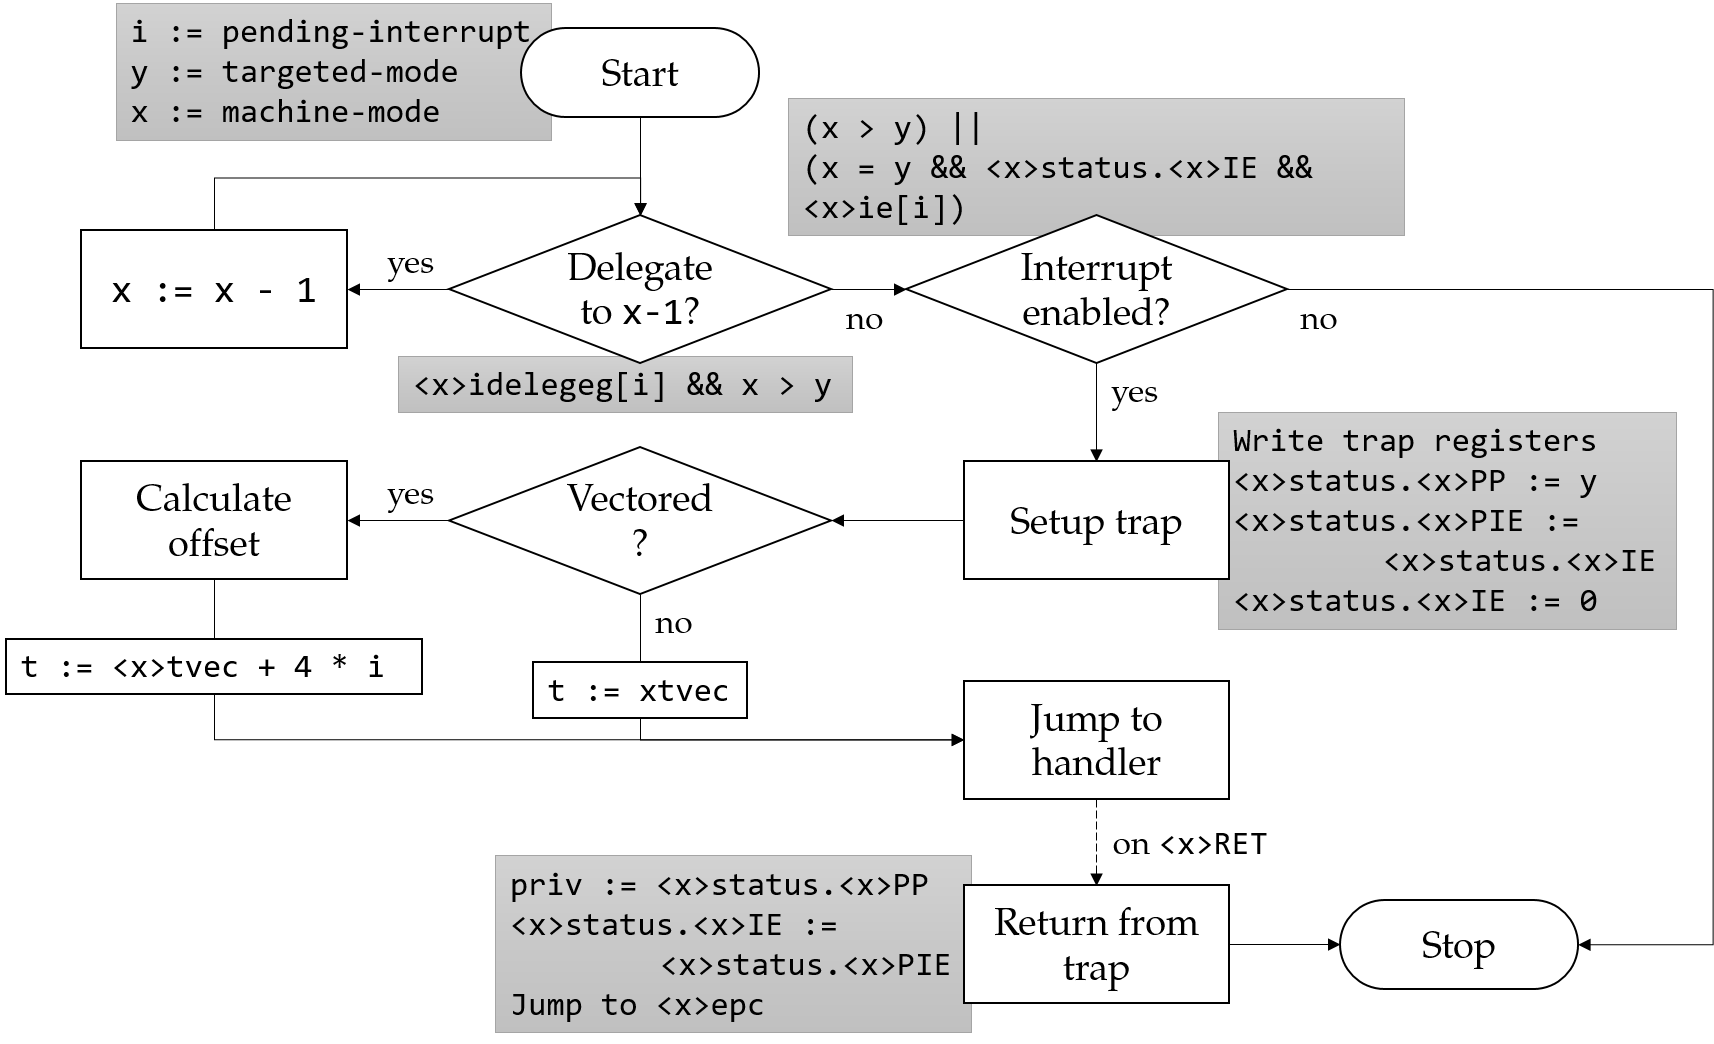
\includegraphics[width=\textwidth]{figures/interrupt-handling.png}
    \caption{Interrupt handling flow-chart}
    \label{fig:interrupt-handling}
\end{figure}

There are three categories of interrupts: external interrupts, timer interrupts and software interrupts.
External interrupts are used to signal exceptional events occurring on some external device that is connected to the core.
Timer interrupts can be used to track time.
Code can use certain \glspl{csr} to signal to the platform that it needs to be alerted when a given amount of real world time has passed.
Such an alert will be given by a timer interrupt.
Software interrupts can be set pending by software running on the same \gls{hart} with equal or higher privilege than the targeted privilege mode.
Software interrupts have no predefined semantics and thus can be used by programmers or system designers in every imaginable way.

Each of these categories of interrupts can target any privilege-mode resulting in a total of six interrupts available to the platform in our case (or nine if supervisor-mode is supported).
These interrupt-types are associated with indices in the range from $ 0_{10} $ to $ 11_{10} $, also called interrupt code\footnote{%
    The reader might have noticed that these are more indices than needed to encode all interrupts available - even if supervisor-mode is present.
    Indices 2, 6 and 10 currently are reserved.
    These indices' two least significant bits are $ 10_2 $ which corresponds to the encoding of hypervisor-mode.
    When hypervisor-mode was removed from the specification, these bits were marked as reserved.
}.
Interrupts can be set pending individually in the \gls{mip} register.
An interrupt is set pending if the bit of the \gls{mip} corresponding to the interrupts index is set to 1.

If an interrupt or exception is set pending, it must first be decided which privilege mode will take the trap to handle the exception generated.
By default, all interrupts and exceptions will be handled by machine-mode.
However, interrupts and exceptions can be delegated to less privileged modes via the \gls{mideleg} and \gls{medeleg} register\footnote{%
    It would also be possible to delegate traps by using the \gls{mret} instruction and setting all corresponding \glspl{csr} accordingly.
    However, this would come with a higher latency as a couple of jumps would need to be performed first.

    Furthermore, if supervisor-mode is supported, there are supervisor-mode equivalents to the \gls{medeleg} and \gls{mideleg} registers to further delegate interrupts and exceptions to user-mode.
}.
Delegation of interrupts can be disabled either by software writing the bits of \gls{mideleg} and \gls{medeleg} accordingly or by an implementation not supporting these registers altogether.
Similar to the \gls{mip} register, each bit field of \gls{mideleg} corresponds to the interrupt of the same index.
Exceptions also have an exception code assigned and thus, fields of \gls{medeleg} correspond to these codes.
An interrupt or exception can only be delegated to modes equally or higher privileged than the mode the interrupt or exception was targeting originally.
For example, if an interrupt is targeting supervisor-mode it can optionally be delegated to supervisor-mode or must be handled by machine-mode but cannot be handled by user-mode.
For each mode $ x $ ($ x \in \{ \text{M}, \text{S}, \text{U}\} $, there are respective counterparts to machine-mode registers such as \gls{mip}, e.g., if an interrupt is delegated to mode $ x $, the corresponding bit in the respective \gls{xip} register reads accordingly and becomes writable.
Otherwise it appears to be hardwired to zero.
From now on, registers related to interrupt and exception handling will be introduced for some arbitrary mode $ x $.

After the mode to be targeted by the trap has been determined, it must be checked whether the given interrupt is actually enabled.
Exceptions cannot be disabled and therefore will always be taken - as a consequence the following checks will be omitted for exceptions.
Interrupts on the other hand can be dis- or enabled individually in the \gls{xie} register.
Analogously to the \gls{xip} register, an interrupt is enabled if the bit corresponding to the interrupt's index is set to 1.
Additionally, the \gls{xstatus} register can globally dis- or enable interrupt handling for a specific mode via its $x$IE bits.
These $x$IE fields, however, are only taken into account if the \gls{hart} operates at an equal or higher privilege mode than targeted, i.e. interrupts are always enabled globally if some interrupt is targeting a mode of higher privilege than the mode of current operation.
Finally, an interrupt will be taken if interrupts are globally enabled \textit{and} the interrupt itself is enabled in the \gls{xie} register.

If a pending interrupt is taken, the \gls{xepc}, \gls{xcause}, \gls{xtval}, and \gls{xstatus} registers are written and the platform will jump to a base address held by the \gls{xtvec} register.
\gls{xtvec} also provides a field that controls whether interrupts can be \textit{vectored}, i.e. for interrupts the \gls{pc} is not set to the base address for handling trap but to $ (\text{base} + 4 \times \text{cause}) $.
\gls{xepc} holds the address of the original instruction stream that was preempted, i.e. either the address of the instruction that caused the exception or the instruction that was next to be executed as a external interrupt was taken.
\gls{xcause} holds an identifier of the current interrupt or exception being handled by the trap.
The most significant bit indicates whether an interrupt is currently being serviced and all other bits hold the exception or interrupt code.
\gls{xtval} serves as a register to hold arguments for a trap handler.
Technically, it holds \textcquote{RiscVISAP}{exception-specific information to assist software in handling the trap}.
One example for such \enquote{exception-specific information} is that \gls{xtval} can contain the faulting bits of an instruction for an illegal instruction exception whereas \gls{xepc} would only point to the instruction in memory as a whole therefore not giving specific information about which part of the instruction caused the exception.

\gls{xstatus} also provides bits to \enquote{stack} certain values when handling exceptions or interrupts.
Firstly, nested interrupts are only supported between privilege modes.
To implement this, on a trap to handle an interrupt in mode $ x $, interrupts are disabled for this mode and the value of the interrupt-enable bit is \enquote{stacked onto} a prior-interrupt-enable bit $x$PIE, i.e. $ x\text{PIE} := x\text{IE} $ and $ x\text{IE} := 0 $.
Secondly, there is a prior-privilege bit $x$PP that stores the privilege mode before the trap was taken.

Note that due to the small offset between vectored interrupt jump destinations, the instructions located there cannot perform more than jumping to the \textit{real} trap handler.
Furthermore, as exceptions cannot be vectored, any differentiation between those must be performed by software.

After the jump to the trap handler, at some point, the $x$RET instruction will be executed signalizing that the trap has been handled sufficiently.
On execution of the $x$RET instruction, the architecture will reset the state according to the values stacked earlier, i.e. \gls{xstatus}.$x$IE is written with \gls{xstatus}.$x$PIE, the privilege mode is set to \gls{xstatus}.$x$PP and the \gls{pc} is set to \gls{xepc} and normal execution continues until the next interrupt or exception occurs.

\paragraph{Summary}
In the previous paragraphs, the basic ideas of the three levels of privilege, memory attributes and protection and interrupt and exception handling specified by the privileged architecture of RISC-V \cite{RiscVISAP} were introduced.
The specification includes even more mechanisms then these, e.g., it was touched that there are timer \glspl{csr} but there is much more.
However, these mechanisms are beyond this thesis's scope as they \begin{enumerate*}[label=\alph*)]
    \item often do not introduce new concepts to the architecture as a whole but build up on already introduced ones\footnote{%
        A prominent exception to this is supervisor-mode adding support for virtualization.
    } and
    \item already exceed what will be incorporated in the MINRV8 architecture.
\end{enumerate*}

To summarize:
\glspl{pma} and \gls{pmp} entries make general properties of physical memory transparent to software allowing it to adopt to possible interactions with respective regions correctly.
\gls{pmp} entries, however, can also be used for memory protection in addition to virtualization.

An overview of all registers that are involved in trap handling can be found in table \ref{tbl:trap-csrs}.
\glspl{csr} which are available to user-mode would also be available to supervisor-mode in this context.
Registers written in italic font are not actual registers on their own but provide a restricted view on their respective machine-mode counterpart.

\begin{table}
    \centering
    \begin{tabular}{| c c || l |}
        \hline
        \textbf{Machine-mode} & \textbf{User-mode} & \textbf{Description} \\
        \acrshort{mstatus} & \textit{\acrshort{ustatus}} & Status \\
        \acrshort{mie} & \textit{\acrshort{uie}} & Interrupt enable \\
        \acrshort{mip} & \textit{\acrshort{uip}} & Interrupt pending \\
        \acrshort{mtvec} & \acrshort{utvec} & Trap-vector base address \\
        \acrshort{mscratch} & \acrshort{uscratch} & Scratch \\
        \acrshort{mepc} & \acrshort{uepc} & Exception program counter \\
        \acrshort{mcause} & \acrshort{ucause} & Trap cause \\
        \acrshort{mtval} & \acrshort{utval} & Trap value \\
        \acrshort{medeleg} & & Exception delegation \\
        \acrshort{mideleg} & & Interrupt delegation \\
        \hline
    \end{tabular}
    \caption{Trap-handling \glspl{csr}}
    \label{tbl:trap-csrs}
\end{table}

Summarizing the mechanisms that play into interrupt and exception handling, recall the four steps to interrupt and exception handling we introduced at the beginning of this section.
These can now be filled with more details:
\begin{enumerate}
    \item If an interrupt or exception is pending, determine the privilege mode to take the trap by checking the targeted privilege mode and any delegation settings
    \item If an interrupt is pending, check that interrupts are enabled globally and check that the specific interrupt is enabled as well
    \item Take the trap by jumping to to trap base vector and if an interrupt is being serviced take vectoring into account
    \item Return from trap handler
\end{enumerate}

The differences between handling exceptions and interrupts can be summarized by the following:
\begin{itemize}
    \item Exception cannot be disabled therefore they will always be handled
    \item $ x\text{cause}[31] $ is written with $ 0 $
    \item Exceptions cannot be vectored therefore the \gls{pc} will always be set to $ x\text{tvec} $
\end{itemize}

To adopt figure \ref{fig:interrupt-handling} accordingly, one would need to alter it by replacing most interrupt-related \glspl{csr} with their exception-related counterpart if possible.
An exception to this is $ x\text{status}.x\text{IE} $ which still is set to 0, meaning that it is not possible to preempt handling an exception by handling an interrupt.

Finally, note that exceptions are handled as soon as they occur.
This is necessary as exceptions always are closely related to the current stream of instructions and therefore need attention before said stream can continue to be executed.
The only exception to this are other interrupts which are handled before any exception with the following decreasing order of priority: external interrupts, software interrupts, timer interrupts, exceptions.
RISC-V knows no concept of settings exceptions pending, this however, is not necessary.
If an exception occurs while an interrupt is set pending, the interrupt can be handled with \gls{xepc} being set to the address of the faulting instruction which either will again fault after the interrupt has been handled or will succeed by some magical condition in which case it does need any further attention\footnote{
    While not being a citable source, credit should be given to Stack Overflow user Baard who pointed this out to us (cf. \url{https://stackoverflow.com/a/56402079/7194995}).
}.

\subsection{Feature Selection}
\label{sec:risc-v-selection}

From what has been introduced of the RISC-V architecture, a selection of features to include in the MINRV8 architecture will now be made.
The overall goal is to create an architecture that is simplified in comparison to the RISC-V \gls{isa} but still incorporates all types of features necessary to introduce a sufficient level of complexity allowing the MINRV8 to be comparable to modern architectures.

The first decision is which combination of privilege levels to model.
In section \ref{sec:rv-priv-arch}, it has been mentioned that in this thesis, the focus will be put on secure embedded systems, i.e. systems supporting user- and machine-mode but not supervisor-mode.
The core features added by supervisor-mode are those of virtualization.
Since we deemed memory virtualization as out of scope in this context (cf. sec. \ref{sec:virtual-memory}), we value simplicity over completeness of the model and rule out supervisor-mode.

Additionally, to keep the state space small, we decided to model an architecture where the word size is eight bit.
There is no reason to believe that an increase in word size introduces fundamentally new security or information flow issues to an architecture so it was decided to value efficiency over completeness in this case.
Since the state space grows exponentially in word size, choosing a smaller word size should significantly improve the performance of the model.

From both parts of the RISC-V specification, the base integer instruction set and the privileged architecture, the MINRV8 architecture will include the very foundation of all categories introduced except jumps and branches.

Consequently, MINRV8 supports integer arithmetic, bitwise-logical instructions and bit-shifts, loads and stores, as well as instructions to read and write \glspl{csr} and to transition between privilege modes.

As for memory attributes, we decided to implement caching mechanisms in the architecture.
Therefore, \glspl{pma} will be given in form of cacheability settings but nothing more.
The RISC-V specification is quite vague when it comes to other types of \glspl{pma}.
It mentions them but does not formally specify their workings.
We interpret this as \glspl{pma} applying more to specific implementations than RISC-V as a whole since each type of \glspl{pma} needs to be specified further when implemented.
Therefore, it was decided to include only \glspl{pma} for which positive reasons can be given - applying only to caching \glspl{pma}.

We adopt \gls{pmp} entries as well.
There will be no configurable but fixed memory regions but each of these can be set readable, writable and locked freely.
The decision towards fixed regions of memory was made during the prototyping phase where we found that dynamic memory regions significantly impacted the performance of the model.

As for interrupts and exceptions, the MINRV8 architecture supports the call to machine-mode exception and external interrupts targeting machine-mode.
An implementation of more types of interrupts adds additional complexity without serving a clear purpose besides the completeness of the model.
Therefore, following the decision on supervisor-mode, simplicity was valued over completeness.
Concerning the interrupt handling routine, it was decided to remove all optional parts from it, i.e. there is no interrupt delegation and there are no vectored interrupts.
Furthermore, as all interrupts target machine mode, there is no need to check the target of an interrupt or exception initially.
This leaves MINRV8 with the following, very simple interrupt/exception handling routine:
\begin{enumerate}
    \item If an interrupt is pending, check that interrupts are enabled globally and the specific interrupt is enabled as well
    \item Take the trap
    \item Return from trap handler
\end{enumerate}

\section{The MINRV8 Architecture}
\label{sec:minrv8}

The architecture that will be model checked in this thesis is a minimal, RISC-V-inspired 8-bit architecture and shall be named MINRV8 from now on.
A secure embedded system that implements the RV32E, i.e. base integer instruction set for embedded computing, was taken as a role model for this minimal architecture.
The reasoning behind the architecture and features included was given in section \ref{sec:risc-v-selection}.
In this section, the architecture itself will be introduced and briefly specified.

MINRV8 supports four general purpose registers and has two privilege modes: machine- and user-mode.
Besides this, it has 4-bytes of readable and writeable but non-executable memory divided into two regions the first of which ranges from addresses 0 to 1 whereas the other occupies the remaining addresses 2 to 3.
MINRV8 supports basic instructions for memory reads and writes, integer arithmetic with $ + $ and $ - $, bit-shifts, bitwise-logical operations with \minrv{And} and \minrv{Or}, a \minrv{Mov} instruction to move a word from one register to another, a comparison instruction, two instructions to switch privilege mode and instructions to read and write \glspl{csr}.
A full list of all instructions can be found in table \ref{tbl:min-arch-instrs}.
Machine words are generally interpreted as signed-words thus there will not be unsigned counterparts to integer arithmetic or the comparison instruction.

With this list of instructions, all instructions of the base integer instruction set of the RISC-V \gls{isa} are either left out deliberately, can be emulated, or have been made redundant by other design decisions of the MINRV8 \gls{isa}.
As for what has been left out, it was already mentioned that jumps and branches will not be modelled.
Since this removes the need for a \gls{pc}, the \gls{auipc} instruction, which is supported by RISC-V, is made redundant as well.
This decision is closely related to the way the MINRV8 architecture was modelled.
In section \ref{sec:minrv8-restrictions}, an outlook on the reasoning behind this will be given.

Additionally, there is the \gls{ebreak} instruction that transfers control to a debugging environment.
It was decided to not include debugging in the MINRV8 architecture since, as mentioned before, at its current state the level of complexity offered by the architecture is sufficient to make it comparable to other modern \gls{risc} architectures.
Finally, there is the FENCE instruction that allows to order memory access.
As the \glspl{pma} do not support memory ordering, this instruction was left out as well.

For most computational instructions, RISC-V offers an immediate alternative that, instead of receiving two registers as arguments, receive one register and one immediate value from memory as arguments.
These instructions can be emulated by first executing the \minrv{Loadi} instruction and then the respective non-immediate version of the instruction.
Also, RISC-V supports the XOR, \gls{srl}, and \gls{csrrw} instructions that can both be emulated.
XOR can be emulated by a combination of \minrv{Sub}\footnote{%
    \minrv{Sub} can be used to implement the bitwise, logical not, i.e. for a bit vector $ x $ of length $ n $, the bitwise, logical not is given by $ 1^n - x $, where $ 1^n $ is the repeated concatenation of bit $ 1 $.
}, \minrv{And}, and \minrv{Or}, \gls{srl} by \minrv{Sll} with a negative argument to shift the register by, and \gls{csrrw} by \minrv{Csrrs} and \minrv{Csrrc} executed subsequently.

Instructions that have been made redundant are all unsigned variants of computational instructions and load/store instructions of word sizes greater than bytes.
These load/store instructions have been made redundant with the decision to limit the word size of MINRV8 to one byte.

All this gives strong assurance that the computational model of MINRV8 does not lack in any major part in comparison to RISC-V.

\begin{table}
    \centering
    \begin{tabular}{|l p{8cm}|}
        \hline
        \minrv{Load rd, rs1} & Load the word stored in memory at the address stored in registers \minrv{rs1} modulo 4 into register \minrv{rd} \\
        \minrv{Store rs1, rs2} & Store the word located in register \minrv{rs2} into memory at address stored in register \minrv{rs1} modulo 4 \\
        \minrv{Loadi rd, imm} & Load the 8-bit immediate value \minrv{imm} into register \minrv{rd} \\
        \minrv{Add rd, rs1, rs2} & Set register \minrv{rd} to the sum of the values in registers \minrv{rs1} and \minrv{rs2} \\
        \minrv{Sub rd, rs1, rs2} & Set register \minrv{rd} to the value of register \minrv{rs1} minus the value of register \minrv{rs2} \\
        \minrv{And rd, rs1, rs2} & Set register \minrv{rd} to the result of a bitwise-and of the values of registers \minrv{rs1} and \minrv{rs2} \\
        \minrv{Or rd, rs1, rs2} & Same as \minrv{And} but with the bitwise-or operation \\
        \minrv{Mov rd, rs1} & Set register \minrv{rd} to the content of register \minrv{rs1} \\
        \minrv{Sll rd, rs1, rs2} & Set register \minrv{rd} to content of register \minrv{rs1} shifted left logically (i.e. without sign-extension) by the value in register \minrv{rs2} \\
        \minrv{Sra rd, rs1, rs2} & Set register \minrv{rd} to the content of register \minrv{rs1} shifted right arithmetically (i.e. with sign-extension) by the value in register \minrv{rs2} \\
        \minrv{Slt rd, rs1, rs2} & Set register \minrv{rd} to 0x01 if the value in register \minrv{rs1} is smaller than the value in register \minrv{rs2} \\
        \minrv{Ecall} & Environment call to machine-mode \\
        \minrv{Mret} & Machine-mode return from trap handler \\
        \minrv{Csrrs rd, rs1, rs2} & Read the value of the \gls{csr} with index \minrv{rs1} modulo the number of all \glspl{csr} and store it in register \minrv{rd}; additionally, set all bits of the \gls{csr} high that are high in register \minrv{rs2} \\
        \minrv{Csrrc rd, rs1, rs2} & Same as \minrv{Csrrs} but set all bits low that are low in register \minrv{rs2} \\
        \hline
    \end{tabular}
    \caption{Instructions of the MINRV8 architecture}
    \label{tbl:min-arch-instrs}
\end{table}

Besides the general purpose storage options, MINRV8 also includes three \glspl{csr}: an \gls{mstatus} equivalent, a \gls{pmpcfg} equivalent and a \gls{pmacfg} register that implements the configuration \glspl{pma} as described in section \ref{sec:risc-v-selection}.
MINRV8 supports external interrupts as the only source of interrupts and an environment call to machine-mode as the only source of exceptions.
Therefore, in the context of MINRV8, \gls{mstatus} has 4 bits comprising two stacking bits for taking traps, i.e. MPP (machine-mode prior privilege) and MPIE (machine-mode prior interrupts enabled), a MEIP bit to signal pending external interrupts and a MIE bit to en- or disable interrupts globally.
By this combination of \glspl{csr}, it was only included from RISC-V what was necessary to implement the features presented in section \ref{sec:risc-v-selection}.

The \gls{pmacfg} register defines cacheability of the two memory regions.
Each memory region can either be set as uncacheable, write-back-cacheable, write-through-cacheable or write-protected-cacheable.
These caching methods are inspired by the caching methods that are available in the x86 architecture from Intel as described in section 11.3 \textit{Methods of Caching Available} of the \citetitle{IntelSystemProgramming} \cite{IntelSystemProgramming}.
This manual describes these methods of caching as follows:
\begin{displaycquote}[p.11-7]{IntelSystemProgramming}
    \begin{description}
        \item[Write-through (WT)] --- \textelp{} Reads come from cache on cache hits; read misses cause cache fills. \textelp{}
        All writes are written to a cache line (when possible) and through to system memory.
        When writing through to memory, invalid cache lines are never filled, and cache lines are either filled or invalidated. \textelp{}
        \item[Write-back (WB)] --- \textelp{} Reads come from cache lines on cache hits; read misses cause cache fills. \textelp{}
        Write misses cause cache line fills \textelp{}, and writes are performed entirely in the cache, when possible. \textelp{}
        The write-back memory type reduces bus traffic by eliminating many unnecessary writes to system memory.
        Writes to a cache line are not immediately forwarded to system memory; instead, they are accumulated in the cache.
        The modified cache lines are written to system memory later, when a write-back operation is performed.
        Write-back operations are triggered when a cache lines need to be deallocated, such as when new cache lines are being allocated in a cache that is already fill. \textelp{}
        \item[Write-protected (WP)] --- Reads come from cache lines when possible, and read misses cause cache fills.
        Writes are propagated to the system bus and cause corresponding cache lines on all processors on the bus to be invalidated.
        \textelp{}
    \end{description}
\end{displaycquote}

Cited paragraphs from the \citetitle{IntelSystemProgramming} are summarized in table \ref{tbl:cache-methods}.
In this setting, it was decided to always fill the cache on write-hits for write-through-cacheable memory regions to make the caching methods as concise as possible although the manual leaves it open to implementations to also invalidate the cache.

\begin{table}
    \centering
    \begin{tabular}{| c r | c c c c |}
        \hline
        && Uncached & WB & WT & WP \\
        \hline
        \multirow{2}{*}{Write} & Hit & \ding{53} & Fill & Fill if valid & Invalidate \\
        & Miss & \ding{53} & Fill & \ding{53} & \ding{53} \\
        \hline
        \multirow{2}{*}{Read} & Hit & \ding{53} & Read & Read & Read \\
        & Miss & \ding{53} & Fill & Fill & Fill \\
        \hline
    \end{tabular}

    {\small \ding{53} = no action}
    \caption{Caching Methods}
    \label{tbl:cache-methods}
\end{table}

The \gls{pmpcfg} register allows to set read and write privileges per memory region and allows to lock the settings of individual regions.

\subsection{Restrictions of the MINRV8 Architecture}
\label{sec:minrv8-restrictions}

Someone experienced in the field of microcontrollers and processors might find MINRV8 to lack the crucial features of jump and branch instructions and the specification of executable memory.
These points were left out or left unspecified deliberately.
The development of the MINRV8 architecture was tightly coupled to its implementation in nuXmv which will presented in section \ref{sec:model-implementation}.
In the implementation, it was decided to model the stream of instructions to the architecture as input variables.
This makes a model of jump and branch instructions or executable memory pointless since input variables cannot be constrained.
A more thorough discussion of this problem will be given in section \ref{sec:discuss-arch} where the scope of the MINRV8 architecture will be analyzed - both in terms of what it tries to achieve and what it actually is capable of representing, i.e. how close it comes to real-life architectures.

\section{Implementation of MINRV8 in nuXmv}
\label{sec:model-implementation}

With the MINRV8 \gls{isa} being set up, this section presents its implementation in nuXmv.
Cf. section \ref{sec:nuxmv} for an introduction to this tool.
The implementation of MINRV8 was split into two modules:
the first module implements the general mechanisms of the \gls{isa} which include everything but caching which is implemented in a separate module.
In analogy to this, section \ref{sec:implementation-core} will describe how the main module was implemented and section \ref{sec:implementation-caching} will explain the implementation of the module related to caching.
In each of these section, the variables and their corresponding types will be stated declared as part of the modules after which the transition relation for each of the respective variables will be outlined.

The goal of this section is not to give a full description of the whole implementation but to give an overall understanding of the core ideas behind it\footnote{%
    If the full implementation is of interest, the repository containing it is accessible via: \url{https://github.com/felixlinker/ifc-rv-thesis}
}.
The implementation includes practical solutions to certain downsides of nuXmv, and generalizations to ease the implementation as a whole.
All these aspects are not relevant for the goal of this thesis.
It should be noted that the macro processing engine pyexpander \cite{pyexpander} was used to remove redundancies.
nuXmv is certainly not the most low-level language imaginable, however, programming nuXmv still lead to many redundancies in the codebase.
pyexpander in principle serves the same purpose as the C-preprocessor but is much more powerful and allowed to get rid of most aforementioned redundancies.

\subsection{Core Functionality}
\label{sec:implementation-core}

\paragraph{Variables}
The core of the MINRV8 architecture is modelled using four variables:
\begin{itemize}
    \item \smv{priv : boolean}
    \item \smv{csrs : array 0..1 of unsigned word[8]}
    \item \smv{regs : array 0..3 of signed word[8]}
    \item \smv{memory : array 0..3 of signed word[8]}
\end{itemize}

As the names suggest: \smv{priv} indicates the current privilege mode where \smv{TRUE} means that the \gls{hart} is in machine-mode and \smv{FALSE} means that the \gls{hart} is in user-mode.
\smv{csrs} hold the three \glspl{csr} of the MINRV8 architecture.
Technically, only 16 bits are needed to implement all \glspl{csr} of the MINRV8 architecture which is why only two \enquote{physical} \glspl{csr} are modelled.
This allows to implement a homogeneous interface for memory/register reads and writes and does not introduce unused bits to the implementation, i.e. dead state space that still requires traversal from nuXmv.
\gls{mstatus} is located in the lower half (bits 0 to 3) of \smv{csrs[0]}, \gls{pmacfg} in the upper half (bits 4 to 7) of \smv{csrs[0]} and \gls{pmpcfg} in \smv{csrs[1]}.
The variables \smv{regs} and \smv{memory} implement the registers and memory in a straight-forward fashion.

Furthermore, the model knows five input variables:
\begin{itemize}
    \item \smv{op}
    \item \smv{rd : 0..3}
    \item \smv{rs1 : 0..3}
    \item \smv{rs2 : 0..3}
    \item \smv{m_external_interrupt : unsigned word[1]}
\end{itemize}

\smv{op}, \smv{rd}, \smv{rs1} and \smv{rs2} represent a fully decoded instruction where \smv{op} is the opcode as a symbolic constant and the other arguments point to registers with per-instruction determined semantics.
When an instruction does not support some or all of the arguments to the instruction, the values of these input variables simply are ignored.
The variable \smv{m_external_interrupt} signals the event of a pending external interrupt from some source outside of the \gls{hart}.

There is no input variable for an immediate value which might be needed by the \minrv{Loadi} instruction because otherwise, extra state space would be wasted.
Instead, the content of the destination register in the case of a \minrv{Loadi} instruction being executed is not constrained.
This means that nuXmv can choose any value in the next state for register \smv{i} if it happens to be targeted by instruction \minrv{Loadi}.
Thereby, the value written to the destination register by the \minrv{Loadi} instruction is encoded implicitly in the transition relation rather than in the state space.

An overview of the implementation's modules is given in figure \ref{fig:modules-overview}.
On the right-hand side, the main module and its variables are depicted.
Arrows indicate whether one variable influences another.
Sometimes, arrows are labeled to indicate the instruction on which a variable changes its value.
Here, \minrv{Comp.} represents computational instructions such as \minrv{Add} and \minrv{Sys.} stands for platform management instructions such as \minrv{Ecall}.

\begin{figure}
    \centering
    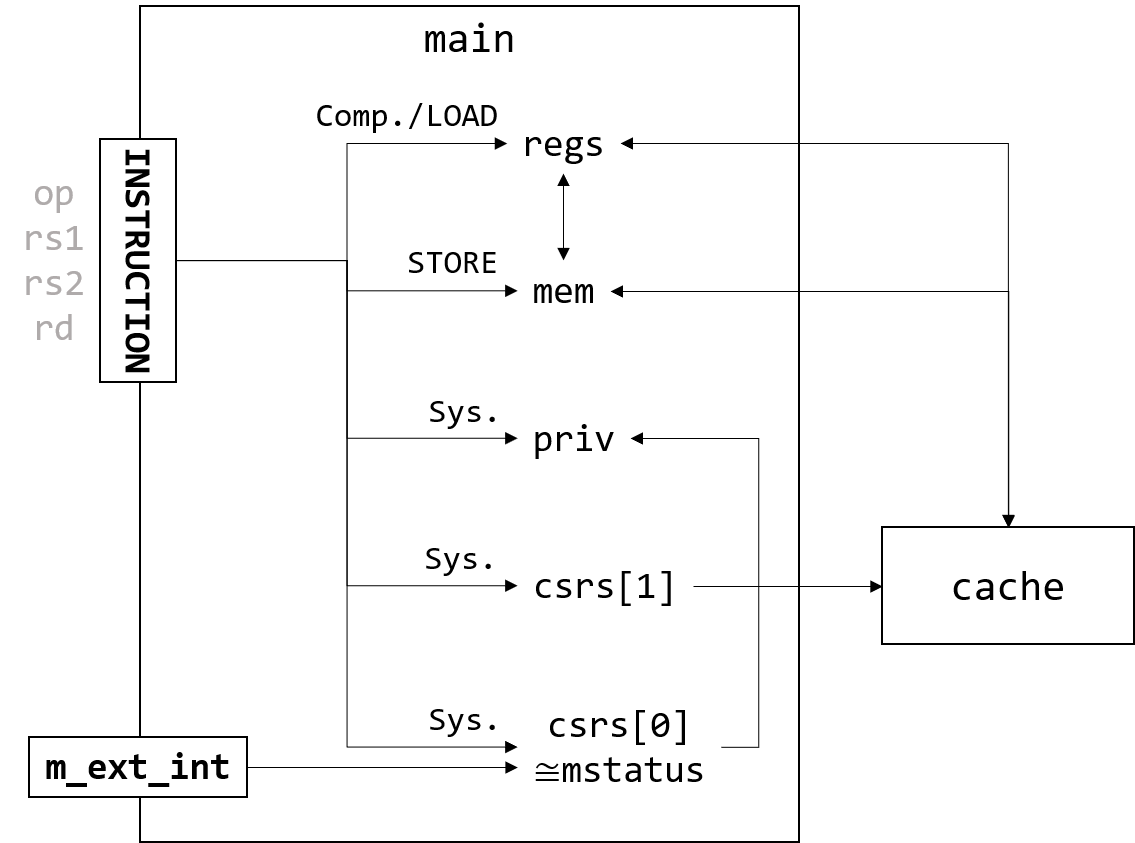
\includegraphics[width=0.7\textwidth]{figures/modules-overview.png}
    \caption{Overview of all modules of the implementation}
    \label{fig:modules-overview}
\end{figure}

\paragraph{Transitions}
nuXmv allows to constrain the transition of variables by arbitrary formulas expressed in propositional logic.
The system can make a transition if it satisfies all formulas given as constraints.
Therefore - if full control over the transition relation is desired - it often is not sufficient to simply constrain transitions by a group of implications\footnote{%
    The exception to this are groups of implications where the antecedents form a total case differentiation, i.e. where one antecedent is always true.
}.
In the implementation for nuXmv of the MINRV8 architecture, \smv{case}-expressions that always close with a default statement were used to ensure that transitions of variables are always fully constrained.

In general, all variables besides \smv{priv} change their value in accordance with the flow-chart depicted in figure \ref{fig:implementation-flow} with some exceptions depending on the variable.
At first, it is checked whether a trap occurred.
All variables besides \smv{mstatus}, which is mapped to \smv{csrs[0]}, are stable in this case.
Then, it is checked whether the current instruction is targeting the respective variable: for example, for an \minrv{Add} instruction, some index \smv{i}, and the variable \smv{regs}, check whether \smv{rd == i}.
Finally, the variable must only change its value, if the current instruction applies to the variable, e.g., a \minrv{Store} instruction will only change values of \minrv{memory} but not \minrv{regs}.
If all checks succeed, the respective instruction is evaluated and the variable is assigned with the instruction's result.

\begin{figure}
    \centering
    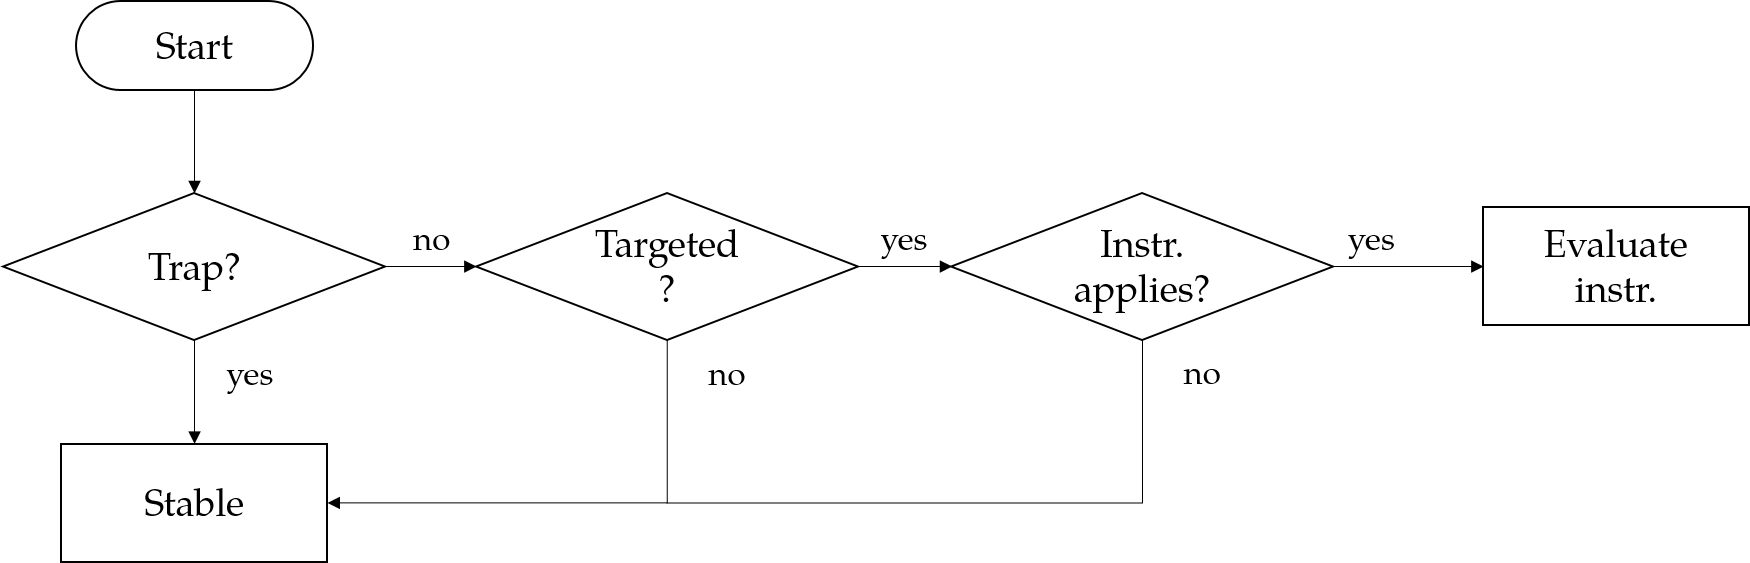
\includegraphics[width=\textwidth]{figures/implementation-flow.png}
    \caption{Variable changing flow-chart}
    \label{fig:implementation-flow}
\end{figure}

In the following, the \enquote{formal idea} of the variable transitions of the model will be introduced.
Whenever there is an exception to the flow-chart depicted in figure \ref{fig:implementation-flow}, it will be made explicit.
Examples for such exceptions are changes of \smv{memory} on cache-line evictions or \smv{mstatus} being influenced by the input variable \smv{m_external_interrupt}.
In this context, it is assumed that variables are stable unless otherwise mentioned.

The transitions of the \smv{priv} variable are simple.
There are two conditions by which \smv{priv} can change.
Firstly, whenever there is an exception - be it an exception triggered by a pending external interrupt or a environment call to machine-mode exception - the \gls{hart} switches to machine-mode and does not execute the current instruction, i.e. the value of \smv{op}, \smv{rd}, \smv{rs1} and \smv{rs2} are ignored.
Secondly, when the \minrv{Mret} instruction is executed, the \gls{hart} sets \smv{priv} to the value stored in \gls{mstatus}.MPP (cf. section \ref{sec:rv-priv-arch}).

\gls{mstatus} changes under the same conditions which leads to the transitions of \smv{csrs}.
On a trap, MPP (machine-mode prior privilege) and MPIE (machine-mode prior interrupts enabled) are written accordingly while MEIP (machine-mode external interrupt pending) and MIE (machine-mode interrupts enabled) are set to zero.
MEIP can be set to zero although the trap might have been triggered by an \minrv{Ecall} instruction because interrupts have higher priority in RISC-V than synchronous exceptions.
To understand why this is correct, there are two cases to consider.
Either an external interrupt was set pending: then it must be serviced immediately and MEIP must be cleared; or it was not set pending: then writing MEIP with 0 does not change the state since MEIP was 0 to begin with.
On return from machine-mode, i.e. execution of \minrv{Mret}, MIE is written with MPIE, MPIE is set to 1 and MPP is set to 0; all other bits are left unchanged.
An exception to the rules mentioned above is the field MEIP which can be set high on every transition based on the value of \smv{m_external_interrupt}.

All \glspl{csr}, \gls{pmacfg}, \gls{pmpcfg}, and partially \gls{mstatus}, can also be written by the \minrv{Csrrc} or \minrv{Csrrs} instructions.
In order to control read- and write-access to the \glspl{csr}, the model knows two constant arrays:
\begin{lstlisting}[language=smv]
    __csrs_read_privs := [ 0h_0F, 0h_00 ];
    __csrs_write_privs := [ 0h_FF, 0h_FF ];
\end{lstlisting}

These arrays provide bitmasks that indicate the least privilege level necessary to read or write the \gls{csr} of the corresponding index at the corresponding bit-position.
All \glspl{csr} besides \gls{mstatus} can be read but but no \gls{csr} can be written by user-mode.
These constants are transformed to the bitmasks \smv{csr_read_mask} or \smv{csr_write_mask} respectively by the per-bit $ b $ implication of $ b \rightarrow \texttt{priv} $ based on the index of the currently targeted \gls{csr}.
Bits of \glspl{csr} are changed by the \minrv{Csrrs} or \minrv{Csrrc} instruction only if \smv{csr_write_mask} is high at the corresponding index with two exceptions:
\begin{itemize}
    \item \gls{mstatus}.MEIP cannot be written by software
    \item Once a \gls{pmpcfg} register has been locked, it cannot be changed anymore
\end{itemize}

The transition relation of the registers and memory is easier to understand.
\smv{regs} changes at index \smv{i} if it is targeted by some instruction and no trap is taken.
Then, \smv{regs[i]} is written with a value determined by the instruction semantics\footnote{%
    This only applies to instructions that \textit{have} semantics targeting registers, e.g., \minrv{Ecall} will not change values of any register.
}.
These per-instruction semantics include considering the \smv{csr_read_mask} bitmask on \minrv{Csrrs} and \minrv{Csrrc}.

\smv{memory} is written at index \smv{i} if it is targeted by the \minrv{Store} instruction, no trap occurs and the write privilege settings in \gls{pmpcfg} allow the current privilege mode to write the register.
Otherwise \smv{memory} does not change.
It does not mark an error, should the current privilege level not suffice to write the targeted memory address.
No exception will be generated - the memory simply will not be written.
The same holds for read privileges and \smv{regs} on a \minrv{Load}.

\subsection{Caching}
\label{sec:implementation-caching}

The cache is implemented as its own module that gets instantiated by the main module.
It increases the complexity of the memory's and registers' transition relation.
The module comprises three variables:
\begin{itemize}
    \item \smv{addr : 0..3}
    \item \smv{valid : boolean}
    \item \smv{line : signed word[8]}
\end{itemize}

The type of the \smv{line} variable indicates that this cache can only store one word, i.e. one byte, at a time.
These variables transition depend on the cache-configuration of the respective memory region in \gls{pmacfg}.
As already introduced in section \ref{sec:minrv8}, a memory region can be either set as uncacheable, write-back-cacheable or write-through-cacheable.
If a memory region is set as uncacheable, the cache will ignore reads and writes to this region and not make any transition.

\paragraph{Reads}
If a memory region is set as cacheable\footnote{%
    In context of this thesis, \enquote{cacheable} means that a memory region is marked as write-back-cacheable, write-through-cacheable or write-protected-cacheable.
}, reads will trigger a cache-fill.
On a \minrv{Load}, if the cache is invalid or currently holds the contents of a different memory address than targeted, \smv{addr} gets written with \smv{regs[rs1] mod 4}, i.e. the address to read from, \smv{valid} becomes \smv{TRUE} and \smv{line} is written with \smv{memory[addr]}\footnote{%
    \smv{addr} here refers to the already updated value of that variable, i.e. \smv{regs[rs1] mod 4}.
}, i.e. the value to read.
This process is independent of the current privilege level, e.g., user-mode attempting to read from a memory address causes a cache-fill regardless of whether user-mode can access the region.
In this case, though, user-mode still will not be able to read the respective word as reads are privileged controlled.

If, however, on a \minrv{Load} the cache already holds the targeted word, is valid and the current mode suffices to read the respective memory address, \smv{line} instead of \smv{memory[regs[rs1] mod 4]} will be written into register \smv{rd}.

\paragraph{Writes}
From the cache's perspective, writes to regions which are set cacheable work the same way, regardless of the specific region's cacheability settings.
For such a region, on a \minrv{Store}, \smv{line} is written with \smv{regs[rs2]}, i.e. the word to write, \smv{address} with \smv{regs[rs1] mod 4}, i.e. the address to write to, and \smv{valid} becomes \smv{TRUE}.
However, if the region is set to be write-through-cacheable, the write will also be reflected in memory whereas for a write-back-cacheable region the write will be reflected in cache only.

This brings the need to persist writes to the cache in memory when cache lines are evicted.
For example, consider the following program:
\begin{lstlisting}[language=minrv8]
    Store 1, 0  # store regs[0] at memory[regs[1] mod 4]
    Load 0, 2   # read memory[regs[2] mod 4] to regs[0]
\end{lstlisting}

In general (i.e. when \minrv{regs[1] mod 4 != regs[2] mod 4}\footnote{%
    If this is not assumed, the \minrv{Load} instruction would simply read the word that has just been written from cache.
    The problematic instances are where the cache line is evicted because of the \minrv{Load} instruction.
}), if the memory region targeted by \minrv{regs[1]} is set to be write-back-cacheable the write in the first line will not be persisted in memory but on cache level only.
If furthermore the memory region targeted by \minrv{regs[2]} is set to be cacheable as well, the read in the second line will overwrite changes of the first instruction which is why the cache content must first be written to memory.
Therefore, if the cache holds some non persisted values of write-back-cacheable memory regions and either the cache's target changes or the \gls{pmacfg} attributes change such that the cache is not write-back-cacheable anymore, the content of the cache will be written to memory as well.

\section{Summary}
\label{sec:arch-summary}

In this section, the core of the RISC-V \gls{isa} was introduced from which the MINRV8 architecture was derived (cf. section \ref{sec:risc-v}).
MINRV8 supports machine- and user-mode as privilege levels and 15 instructions to perform general computation, read/write memory, load immediate values from memory, transition between privilege modes and read/write \glspl{csr} (cf. table \ref{tbl:min-arch-instrs}).
It was shown that this list of instructions is complete in comparison to RISC-V minus very few but negligible instructions that were not included and modulo instructions made redundant by design decisions or that can be emulated.
Furthermore, MINRV8 supports caching of memory regions and \gls{pmp} entries for memory regions, i.e. read- and write-permissions configurable for user-mode and to some extent for machine-mode (cf. section \ref{sec:minrv8}).

It was argued that MINRV8 provides a sufficient amount of complexity to make it comparable to modern \gls{risc} architectures besides not including a model of executable memory and not supporting jumps and branches.
This will be discussed in section \ref{sec:discuss-arch} and is related to the decision to model the stream of instructions as input variables in nuXmv.

Finally, it was presented how MINRV8 was implemented in nuXmv (cf. section \ref{sec:model-implementation}).
The implementation was conducted by hand with aid of the preprocessor engine pyexpander \cite{pyexpander}.
The file containing the model overall includes 630 lines of code where for the most part no line exceeded 80 characters.
